\chapter{Cookie e Preferenze}\label{cap:cookie}

\begin{tcolorbox}[title=Obiettivi del capitolo]
Dopo questo capitolo saprai:
\begin{itemize}
  \item Comprendere cosa sono i cookie e come funzionano nel protocollo HTTP
  \item Configurare cookie con opzioni di sicurezza adeguate (HttpOnly, Secure, SameSite)
  \item Leggere, validare e serializzare valori cookie in sicurezza
  \item Implementare pattern comuni: preferenze utente, remember me, tracking
  \item Gestire limiti e problemi comuni dei cookie
  \item Applicare best practices per sicurezza e privacy
\end{itemize}
\end{tcolorbox}

\section{Teoria}

\subsection{Cosa sono i cookie}
I cookie sono \textbf{piccoli file di testo} (max 4KB) salvati nel browser dell'utente e inviati automaticamente dal browser al server in ogni richiesta HTTP che corrisponde a path e domain specificati.

\textbf{Caratteristiche chiave}:
\begin{itemize}
  \item \textbf{Persistenza}: Possono durare minuti o anni (o essere cancellati alla chiusura browser)
  \item \textbf{Storage client-side}: Salvati sul dispositivo utente (non sul server)
  \item \textbf{Invio automatico}: Browser li invia in ogni richiesta HTTP al dominio corrispondente
  \item \textbf{Limite dimensione}: Max 4KB per cookie, ~50 cookie per dominio
  \item \textbf{Visibilità utente}: Utente può visualizzare, modificare, cancellare cookie dal browser
\end{itemize}

\subsection{Cookie vs Session vs LocalStorage}

\textbf{Cookie}:
\begin{itemize}
  \item Storage: Client (browser)
  \item Dimensione: Max 4KB
  \item Invio: Automatico in ogni HTTP request
  \item Scadenza: Configurabile (sessione o data specifica)
  \item Accesso JS: Configurabile (HttpOnly flag)
  \item Uso tipico: Autenticazione, preferenze, tracking
\end{itemize}

\textbf{Session} (PHP):
\begin{itemize}
  \item Storage: Server (file, database, Redis)
  \item Dimensione: Illimitata (pratica: MB)
  \item Invio: Solo session ID via cookie
  \item Scadenza: Timeout server-side
  \item Accesso JS: No (dati solo server-side)
  \item Uso tipico: Dati sensibili, carrello, auth state
\end{itemize}

\textbf{LocalStorage/SessionStorage}:
\begin{itemize}
  \item Storage: Client (browser)
  \item Dimensione: 5-10MB
  \item Invio: Mai (solo client-side)
  \item Scadenza: Permanente (LocalStorage) o sessione (SessionStorage)
  \item Accesso JS: Sempre
  \item Uso tipico: Cache client, app state, offline data
\end{itemize}

\subsection{Quando usare i cookie}

I cookie sono particolarmente appropriati per diversi casi d'uso. Sono ideali per l'archiviazione del Session ID utilizzato nell'autenticazione degli utenti, permettendo al server di identificare chi è connesso. Sono anche utili per memorizzare le preferenze utente come il tema dell'interfaccia (chiaro/scuro), la lingua preferita e il layout preferito. I cookie abilitano facilmente la funzionalità "Remember me" che permette agli utenti di rimanere connessi automaticamente. Sono inoltre comunemente utilizzati per il tracking analytics, permettendo ai servizi di analisi di tracciare il comportamento degli utenti. Infine, i cookie possono essere usati per memorizzare il carrello acquisti in siti e-commerce quando l'utente non è autenticato.

D'altro canto, ci sono casi in cui i cookie dovrebbero essere evitati. Non dovrebbero mai essere utilizzati per archiviare dati sensibili non cifrati come password o numeri di carte di credito, poiché sarebbero facilmente vulnerabili al furto. Non dovrebbero contenere dati grandi superiori ai 4KB, il limite dimensionale dei cookie, rendendo il loro trasferimento inefficiente. Dati che non hanno alcun bisogno di essere inviati al server per ogni richiesta (come lo stato dell'interfaccia) dovrebbero essere archiviati in LocalStorage invece che in cookie. Infine, i token anti-CSRF dovrebbero essere memorizzati in sessione lato server piuttosto che come cookie diretto, per evitare che siano facilmente accessibili.

\section{Ciclo di vita dei Cookie}

I cookie seguono un ciclo preciso tra client (browser) e server:

\begin{center}
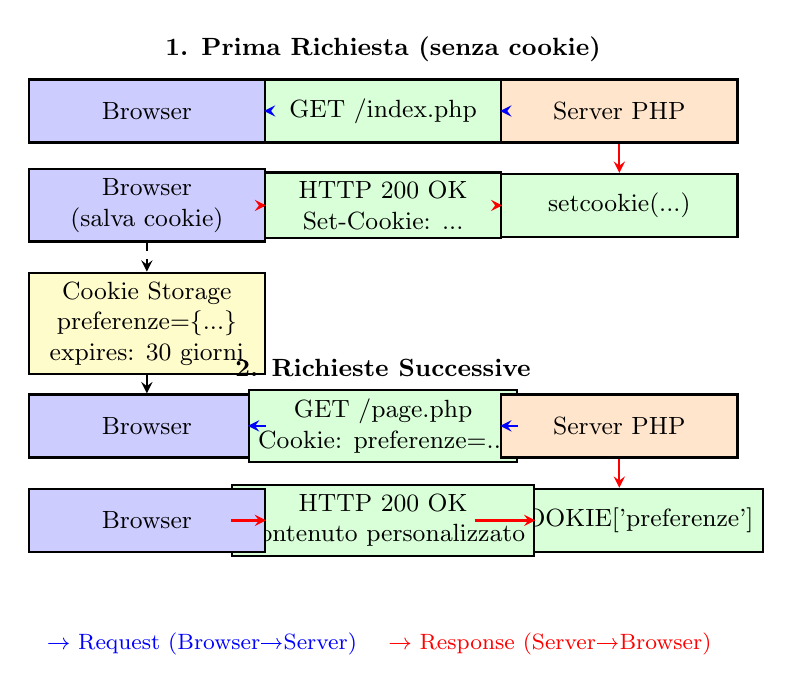
\begin{tikzpicture}[
    node distance=1.5cm,
    box/.style={rectangle, draw, thick, minimum width=3cm, minimum height=0.8cm, align=center, font=\small},
    client/.style={box, fill=blue!20},
    server/.style={box, fill=orange!20},
    action/.style={box, fill=green!15},
    arrow/.style={->, thick, >=stealth}
]
    % Prima richiesta
    \node[above, font=\small\bfseries] at (3,6.5) {1. Prima Richiesta (senza cookie)};

    \node[client] (browser1) at (0,6) {Browser};
    \node[action] (req1) at (3,6) {GET /index.php};
    \node[server] (server1) at (6,6) {Server PHP};

    \draw[arrow, blue] (browser1) -- (req1);
    \draw[arrow, blue] (req1) -- (server1);

    % Set-Cookie Response
    \node[action] (setcookie) at (6,4.8) {setcookie(...)};
    \node[action] (response1) at (3,4.8) {HTTP 200 OK\\Set-Cookie: ...};
    \node[client] (browser2) at (0,4.8) {Browser\\(salva cookie)};

    \draw[arrow, red] (server1) -- (setcookie);
    \draw[arrow, red] (setcookie) -- (response1);
    \draw[arrow, red] (response1) -- (browser2);

    % Storage
    \node[client, fill=yellow!20] (storage) at (0,3.3) {Cookie Storage\\preferenze=\{...\}\\expires: 30 giorni};

    \draw[arrow, dashed] (browser2) -- (storage);

    % Seconda richiesta
    \node[above, font=\small\bfseries] at (3,2.5) {2. Richieste Successive};

    \node[client] (browser3) at (0,2) {Browser};
    \node[action] (req2) at (3,2) {GET /page.php\\Cookie: preferenze=...};
    \node[server] (server2) at (6,2) {Server PHP};

    \draw[arrow] (storage) -- (browser3);
    \draw[arrow, blue] (browser3) -- (req2);
    \draw[arrow, blue] (req2) -- (server2);

    % Read Cookie
    \node[action] (readcookie) at (6,0.8) {\$\_COOKIE['preferenze']};
    \node[action] (response2) at (3,0.8) {HTTP 200 OK\\Contenuto personalizzato};
    \node[client] (browser4) at (0,0.8) {Browser};

    \draw[arrow, red] (server2) -- (readcookie);
    \draw[arrow, red] (readcookie) -- (response2);
    \draw[arrow, red] (response2) -- (browser4);

    % Legenda
    \node[below, font=\footnotesize, align=left] at (3,-0.5) {
        \textcolor{blue}{$\rightarrow$ Request (Browser→Server)} \quad
        \textcolor{red}{$\rightarrow$ Response (Server→Browser)}
    };
\end{tikzpicture}
\end{center}

\begin{tcolorbox}[colback=blue!10, colframe=blue!60, title=Punti chiave del ciclo di vita]
\begin{enumerate}
    \item \textbf{Prima richiesta}: Il browser richiede una pagina senza cookie
    \item \textbf{Set-Cookie}: Il server usa \texttt{setcookie()} per inviare un cookie nella risposta HTTP
    \item \textbf{Storage locale}: Il browser salva il cookie con le sue impostazioni (scadenza, path, domain, flags)
    \item \textbf{Richieste successive}: Il browser invia automaticamente il cookie in ogni richiesta che corrisponde a path/domain
    \item \textbf{Lettura server}: Il server legge il cookie da \texttt{\$\_COOKIE} e personalizza la risposta
\end{enumerate}
\end{tcolorbox}

\section{Impostazione cookie}

\subsection{Sintassi base}
\begin{lstlisting}
<?php
// Sintassi moderna (PHP 7.3+, array opzioni)
setcookie('nome', 'valore', [
    'expires' => time() + 3600,      // Scadenza (Unix timestamp)
    'path' => '/',                   // Path (default: /)
    'domain' => '',                  // Domain (default: dominio corrente)
    'secure' => true,                // Solo HTTPS
    'httponly' => true,              // No accesso JavaScript
    'samesite' => 'Lax'              // CSRF protection (Strict|Lax|None)
]);

// Sintassi vecchia (PHP < 7.3, parametri posizionali)
setcookie('nome', 'valore', time() + 3600, '/', '', true, true);
?>
\end{lstlisting}

\subsection{Attributi cookie}

\textbf{expires} (Unix timestamp): Questo attributo controlla la scadenza del cookie e accetta un timestamp Unix. Se omesso o impostato a 0, il cookie diventa un cookie di sessione e viene automaticamente eliminato quando l'utente chiude il browser. Per impostare una durata specifica, si utilizza \texttt{time() + 3600} per farlo scadere tra 1 ora, \texttt{time() + 86400} per una durata di 1 giorno, o \texttt{time() + 86400 * 30} per 30 giorni. Se si desidera eliminare un cookie esistente, si imposta \texttt{time() - 1} per un timestamp nel passato.

\textbf{path} (string): Questo attributo define il percorso nel dominio dove il cookie è valido. Impostando \texttt{'/'} si rende il cookie valido per l'intero dominio, mentre \texttt{'/admin'} lo rende disponibile solo sotto il path /admin e suoi sottopercorsi. Se non specificato, il default è il path della pagina corrente.

\textbf{domain} (string): Controlla per quale dominio è valido il cookie. La stringa vuota \texttt{''} indica il dominio corrente (comportamento default). È possibile specificare \texttt{'.example.com'} per renderlo valido per tutti i sottodomini di example.com. Per motivi di sicurezza, il browser impedisce di impostare cookie per domini diversi da quello corrente.

\textbf{secure} (bool): Questo flag booleano determina se il cookie viene trasmesso tramite HTTPS o no. Quando impostato a \texttt{true}, il cookie è trasmesso SOLO su HTTPS, proteggendo la riservatezza in transito. Impostando a \texttt{false}, il cookie viene trasmesso anche su HTTP non criptato, opzione rischiosa per dati sensibili. È buona pratica impostare SEMPRE \texttt{secure = true} per cookie di sessione e per cookie contenenti dati sensibili.

\textbf{httponly} (bool): Questo flag determina l'accessibilità del cookie da parte di JavaScript. Quando impostato a \texttt{true}, il cookie NON è accessibile tramite \texttt{document.cookie} in JavaScript, mitigando il rischio di furto tramite XSS. Se impostato a \texttt{false}, JavaScript può leggere e scrivere il cookie liberamente. Per i cookie di sessione, è fondamentale impostare SEMPRE \texttt{httponly = true} per prevenire il furto del session ID tramite attacchi XSS.

\textbf{samesite} (string): Questo attributo controlla il comportamento del cookie in richieste cross-site. \texttt{'Strict'} è l'impostazione più rigorosa e impedisce completamente l'invio del cookie in richieste cross-site, offrendo la massima protezione da CSRF ma potendo causare inconvenienti di usabilità. \texttt{'Lax'} rappresenta un compromesso, inviando il cookie solo in navigazioni top-level GET (come clicare su un link), garantendo un buon equilibrio tra sicurezza e usabilità. \texttt{'None'} consente sempre l'invio del cookie, utile per integrazioni cross-site, ma richiede che \texttt{secure = true} sia impostato.

\subsection{Esempi pratici impostazione}
\begin{lstlisting}
<?php
// Cookie di sessione (cancellato alla chiusura browser)
setcookie('temp_id', uniqid(), [
    'path' => '/',
    'httponly' => true,
    'secure' => true,
    'samesite' => 'Lax'
]);

// Cookie persistente (30 giorni)
setcookie('user_preferences', json_encode(['theme' => 'dark']), [
    'expires' => time() + 86400 * 30,
    'path' => '/',
    'httponly' => false,  // JavaScript può leggere per applicare tema
    'secure' => true,
    'samesite' => 'Lax'
]);

// Session cookie sicuro (autenticazione)
setcookie('PHPSESSID', session_id(), [
    'expires' => 0,  // Sessione (cancellato alla chiusura)
    'path' => '/',
    'httponly' => true,  // SEMPRE true per session
    'secure' => true,    // SEMPRE true per session
    'samesite' => 'Lax'  // O Strict per max sicurezza
]);

// Cancellazione cookie (expires nel passato)
setcookie('old_cookie', '', [
    'expires' => time() - 3600,  // 1 ora fa
    'path' => '/'
]);
?>
\end{lstlisting}

\section{Lettura cookie}

\subsection{Accesso base}
\begin{lstlisting}
<?php
// Leggi cookie (disponibile in $_COOKIE superglobal)
$theme = $_COOKIE['theme'] ?? 'light';  // Fallback se non esiste

// Verifica esistenza
if (isset($_COOKIE['user_id'])) {
    $userId = (int) $_COOKIE['user_id'];
    echo "Utente: $userId";
} else {
    echo "Utente non riconosciuto";
}

// Array di tutti i cookie
print_r($_COOKIE);
?>
\end{lstlisting}

\subsection{Validazione e sanitizzazione}
\begin{lstlisting}
<?php
// SEMPRE validare input da cookie (controllato dall'utente!)

// Validazione stringa semplice
$theme = $_COOKIE['theme'] ?? 'light';
$allowedThemes = ['light', 'dark', 'auto'];
if (!in_array($theme, $allowedThemes, true)) {
    $theme = 'light';  // Fallback sicuro
}

// Validazione numero
$userId = isset($_COOKIE['user_id']) ? (int) $_COOKIE['user_id'] : 0;
if ($userId <= 0) {
    $userId = null;  // Invalido
}

// Validazione pattern (regex)
$lang = $_COOKIE['lang'] ?? 'en';
if (!preg_match('/^[a-z]{2}$/', $lang)) {
    $lang = 'en';  // Fallback se formato errato
}

// Output sanitizzazione (SEMPRE htmlspecialchars per output HTML)
echo htmlspecialchars($_COOKIE['username'] ?? 'Guest', ENT_QUOTES, 'UTF-8');
?>
\end{lstlisting}

\subsection{Deserializzazione JSON}
\begin{lstlisting}
<?php
// Cookie con dati strutturati (JSON)
$defaultPrefs = ['theme' => 'light', 'lang' => 'en', 'notifications' => true];

if (isset($_COOKIE['preferences'])) {
    $prefs = json_decode($_COOKIE['preferences'], true);

    // Valida JSON e struttura
    if (json_last_error() === JSON_ERROR_NONE && is_array($prefs)) {
        // Merge con default (previene chiavi mancanti)
        $prefs = array_merge($defaultPrefs, $prefs);

        // Valida ogni campo
        if (!in_array($prefs['theme'], ['light', 'dark'], true)) {
            $prefs['theme'] = 'light';
        }
        if (!preg_match('/^[a-z]{2}$/', $prefs['lang'])) {
            $prefs['lang'] = 'en';
        }
    } else {
        $prefs = $defaultPrefs;  // JSON corrotto
    }
} else {
    $prefs = $defaultPrefs;  // Cookie non esiste
}

echo "Tema: " . htmlspecialchars($prefs['theme']);
?>
\end{lstlisting}

\section{Sicurezza cookie}

\subsection{Minacce principali}

I cookie sono esposti a diverse minacce di sicurezza che è importante comprendere e mitigare. \textbf{XSS (Cross-Site Scripting)} rappresenta una minaccia significativa dove un attaccante inietta codice JavaScript malicioso che può leggere \texttt{document.cookie} e rubare i cookie di sessione, permettendo all'attaccante di impersonare l'utente. La difesa principale è impostare \texttt{httponly = true} in modo che il cookie non sia accessibile a JavaScript. \textbf{CSRF (Cross-Site Request Forgery)} sfrutta il fatto che il browser invia automaticamente i cookie in richieste cross-site verso il tuo sito da parte di siti malevoli. Un attaccante può così far compiere azioni non autorizzate a nome dell'utente autenticato. La difesa è impostare \texttt{samesite = 'Lax'} o \texttt{'Strict'} per controllare quando il cookie viene inviato. \textbf{Man-in-the-Middle (MITM)} è un attacco dove un attaccante intercetta il traffico HTTP non criptato, riuscendo a leggere o modificare i cookie in transito. La difesa è impostare \texttt{secure = true} in modo che il cookie sia trasmesso solo su HTTPS criptato. \textbf{Session Fixation} è un attacco dove l'attaccante impone un session ID noto all'utente, poi attende che l'utente si autentichi con quel session ID, permettendo all'attaccante di accedere come utente autenticato. La difesa è rigenerare il session ID dopo login utilizzando \texttt{session\_regenerate\_id()}.

\subsection{Cookie sicuri per autenticazione}
\begin{lstlisting}
<?php
// SEMPRE usare questo pattern per session cookie
session_set_cookie_params([
    'lifetime' => 0,              // Sessione (chiusura browser)
    'path' => '/',
    'domain' => '',
    'secure' => true,             // SOLO HTTPS
    'httponly' => true,           // NO JavaScript
    'samesite' => 'Lax'           // CSRF protection
]);

session_start();

// Dopo login, rigenera session ID (previene session fixation)
if ($loginSuccess) {
    session_regenerate_id(true);  // true = cancella vecchia sessione
    $_SESSION['user_id'] = $userId;
    $_SESSION['authenticated'] = true;
}
?>
\end{lstlisting}

\begin{attenzione}
I cookie sono \textbf{sempre inviati automaticamente} dal browser per ogni richiesta al dominio corrispondente. Questo rende necessari i flag di sicurezza:
\begin{itemize}
    \item \textbf{HttpOnly}: Previene accesso JavaScript (protezione XSS)
    \item \textbf{Secure}: Trasmissione solo su HTTPS (protezione man-in-the-middle)
    \item \textbf{SameSite}: Limita invio cross-site (protezione CSRF)
\end{itemize}
\end{attenzione}

\section{Pattern comuni}

\subsection{Remember Me}
\begin{lstlisting}
<?php
// Login con "remember me"
if ($loginSuccess && $_POST['remember_me']) {
    // Genera token sicuro
    $selector = bin2hex(random_bytes(16));
    $validator = bin2hex(random_bytes(32));

    // Hash validator prima di salvare in DB
    $hashedValidator = hash('sha256', $validator);

    // Salva in database
    $db->query(
        "INSERT INTO remember_tokens (user_id, selector, hashed_validator, expires)
         VALUES (?, ?, ?, DATE_ADD(NOW(), INTERVAL 30 DAY))",
        [$userId, $selector, $hashedValidator]
    );

    // Imposta cookie con selector:validator
    setcookie('remember', $selector . ':' . $validator, [
        'expires' => time() + 86400 * 30,
        'path' => '/',
        'httponly' => true,
        'secure' => true,
        'samesite' => 'Lax'
    ]);
}

// Verifica remember token
if (!isset($_SESSION['user_id']) && isset($_COOKIE['remember'])) {
    [$selector, $validator] = explode(':', $_COOKIE['remember'], 2);

    $token = $db->query(
        "SELECT user_id, hashed_validator FROM remember_tokens
         WHERE selector = ? AND expires > NOW()",
        [$selector]
    )->fetch();

    if ($token && hash_equals($token['hashed_validator'], hash('sha256', $validator))) {
        // Token valido: autentica utente
        session_regenerate_id(true);
        $_SESSION['user_id'] = $token['user_id'];
    } else {
        // Token invalido: cancella cookie
        setcookie('remember', '', ['expires' => time() - 3600, 'path' => '/']);
    }
}
?>
\end{lstlisting}

\subsection{Preferenze utente}
\begin{lstlisting}
<?php
// Salva preferenze (tema, lingua, layout)
class UserPreferences {
    private array $defaults = [
        'theme' => 'light',
        'lang' => 'en',
        'layout' => 'grid',
        'notifications' => true
    ];

    public function get(): array {
        if (!isset($_COOKIE['prefs'])) {
            return $this->defaults;
        }

        $prefs = json_decode($_COOKIE['prefs'], true);

        if (json_last_error() !== JSON_ERROR_NONE || !is_array($prefs)) {
            return $this->defaults;
        }

        // Merge con default e valida
        $prefs = array_merge($this->defaults, $prefs);
        $prefs['theme'] = in_array($prefs['theme'], ['light', 'dark'], true)
            ? $prefs['theme'] : 'light';
        $prefs['lang'] = preg_match('/^[a-z]{2}$/', $prefs['lang'])
            ? $prefs['lang'] : 'en';
        $prefs['layout'] = in_array($prefs['layout'], ['grid', 'list'], true)
            ? $prefs['layout'] : 'grid';

        return $prefs;
    }

    public function set(array $prefs): bool {
        $prefs = array_merge($this->defaults, $prefs);
        $json = json_encode($prefs);

        return setcookie('prefs', $json, [
            'expires' => time() + 86400 * 365,  // 1 anno
            'path' => '/',
            'httponly' => false,  // JavaScript può leggere per applicare tema
            'secure' => true,
            'samesite' => 'Lax'
        ]);
    }
}

// Uso
$prefs = new UserPreferences();
$currentPrefs = $prefs->get();
echo "Tema: " . htmlspecialchars($currentPrefs['theme']);

// Update
$prefs->set(['theme' => 'dark', 'lang' => 'it']);
?>
\end{lstlisting}

\subsection{Cookie cifrati (dati sensibili)}
\begin{lstlisting}
<?php
// Cifratura cookie con OpenSSL (per dati sensibili)
class EncryptedCookie {
    private string $key;

    public function __construct() {
        // Chiave segreta (32 byte per AES-256)
        $this->key = hex2bin(getenv('COOKIE_ENCRYPTION_KEY'));
    }

    public function set(string $name, string $value, array $options = []): bool {
        $encrypted = $this->encrypt($value);
        return setcookie($name, $encrypted, $options);
    }

    public function get(string $name): ?string {
        if (!isset($_COOKIE[$name])) {
            return null;
        }

        return $this->decrypt($_COOKIE[$name]);
    }

    private function encrypt(string $plaintext): string {
        $iv = random_bytes(16);  // IV casuale
        $ciphertext = openssl_encrypt($plaintext, 'aes-256-cbc', $this->key, 0, $iv);
        return base64_encode($iv . $ciphertext);
    }

    private function decrypt(string $encrypted): ?string {
        $data = base64_decode($encrypted);
        $iv = substr($data, 0, 16);
        $ciphertext = substr($data, 16);

        $plaintext = openssl_decrypt($ciphertext, 'aes-256-cbc', $this->key, 0, $iv);
        return $plaintext !== false ? $plaintext : null;
    }
}

// Uso
$cookie = new EncryptedCookie();
$cookie->set('sensitive_data', 'secret value', [
    'expires' => time() + 3600,
    'httponly' => true,
    'secure' => true,
    'samesite' => 'Lax'
]);

$value = $cookie->get('sensitive_data');
?>
\end{lstlisting}

\section{Troubleshooting}

\textbf{Problema}: Warning "Cannot modify header information - headers already sent"
\begin{itemize}
  \item \texttt{setcookie()} deve essere chiamato PRIMA di qualsiasi output (HTML, echo, whitespace)
  \item Verifica che non ci sia output prima di \texttt{<?php}
  \item Usa \texttt{ob\_start()} all'inizio dello script se necessario
\end{itemize}

\textbf{Problema}: Cookie non viene impostato
\begin{itemize}
  \item Verifica che non ci sia output prima di \texttt{setcookie()}
  \item Controlla che \texttt{expires} non sia nel passato
  \item Se \texttt{secure = true}, verifica che sito sia HTTPS
  \item Verifica che \texttt{path} e \texttt{domain} corrispondano
\end{itemize}

\textbf{Problema}: Cookie viene cancellato subito
\begin{itemize}
  \item Browser in modalità privata cancella cookie alla chiusura
  \item Utente ha bloccato cookie nelle impostazioni
  \item \texttt{expires = 0} crea session cookie (cancellato alla chiusura)
\end{itemize}

\textbf{Problema}: Cookie non viene inviato in richieste cross-site
\begin{itemize}
  \item \texttt{samesite = 'Strict'} blocca invio cross-site
  \item Usa \texttt{'Lax'} per permettere navigazioni GET
  \item Usa \texttt{'None'} solo se necessario (richiede \texttt{secure = true})
\end{itemize}

\begin{tcolorbox}[title=Best practices]
\begin{itemize}
  \item SEMPRE \texttt{httponly = true} e \texttt{secure = true} per session cookie
  \item Usa \texttt{samesite = 'Lax'} come default (bilanciamento sicurezza/UX)
  \item Valida e sanitizza TUTTI i valori cookie (controllati dall'utente)
  \item Limita dimensione cookie (max 4KB, idealmente < 1KB)
  \item Non salvare dati sensibili in cookie (o cifra con OpenSSL)
  \item Imposta \texttt{expires} esplicito (non fare affidamento su default)
  \item Usa JSON per dati strutturati (con validazione)
  \item Rigenera session ID dopo login (\texttt{session\_regenerate\_id()})
  \item Usa HTTPS in produzione (necessario per \texttt{secure = true})
  \item Informa utenti su uso cookie (GDPR compliance)
\end{itemize}
\end{tcolorbox}

\begin{tcolorbox}[title=Errori comuni]
\begin{itemize}
  \item Output HTML prima di \texttt{setcookie()} (headers already sent)
  \item \texttt{httponly = false} per session cookie (vulnerabile a XSS)
  \item \texttt{secure = false} in produzione (vulnerabile a MITM)
  \item Non validare valori cookie (XSS, injection)
  \item Salvare password o token in chiaro in cookie
  \item Dimenticare \texttt{htmlspecialchars()} quando output cookie
  \item Usare \texttt{samesite = 'None'} senza motivo (espone a CSRF)
  \item Non impostare \texttt{path} (cookie accessibile solo da directory corrente)
  \item Cookie > 4KB (troncato o rifiutato dal browser)
  \item Non gestire caso "cookie non esiste" (causa Notice/Warning)
\end{itemize}
\end{tcolorbox}

\section{Esercizi}

\subsection{Livello base}
\begin{itemize}
  \item Implementa sistema preferenze tema (light/dark) con cookie persistente 30 giorni
  \item Crea contatore visite con cookie, mostra "Prima visita" o "Visita \#N"
  \item Salva lingua preferita (it, en, es) in cookie e applica a interfaccia
\end{itemize}

\subsection{Livello intermedio}
\begin{itemize}
  \item Implementa "Remember me" con token selector/validator salvato in database
  \item Crea sistema preferenze completo (tema, lingua, layout, notifiche) con JSON
  \item Implementa cookie consent banner con preferenze (analytics, marketing, necessari)
\end{itemize}

\subsection{Livello avanzato}
\begin{itemize}
  \item Implementa cookie cifrati con OpenSSL per salvare dati sensibili
  \item Crea sistema A/B testing con cookie che assegna variante (A o B) persistentemente
  \item Implementa cookie-based shopping cart con validazione quantità e prodotti
\end{itemize}

\section{Verifica}

\begin{itemize}
  \item Qual è la dimensione massima di un cookie?
  \item Quali flag sono indispensabili per cookie di autenticazione?
  \item Quando \texttt{SameSite=Strict} può causare problemi e quale alternativa usare?
  \item Differenza tra cookie di sessione e cookie persistente?
  \item Perché \texttt{httponly = true} è importante per session cookie?
  \item Come prevenire session fixation attack?
  \item Cosa succede se chiami \texttt{setcookie()} dopo output HTML?
  \item Quando usare cookie vs session vs LocalStorage?
\end{itemize}

\section{Riferimenti}
\begin{itemize}
  \item RFC 6265 — HTTP State Management Mechanism: \url{https://tools.ietf.org/html/rfc6265}
  \item OWASP — Session Management: \url{https://owasp.org/www-project-web-security-testing-guide/}
  \item PHP setcookie() documentation: \url{https://www.php.net/manual/en/function.setcookie.php}
  \item SameSite Cookies Explained: \url{https://web.dev/samesite-cookies-explained/}
\end{itemize}
